

\tikzset{every picture/.style={line width=0.75pt}} %set default line width to 0.75pt        
\begin{center}
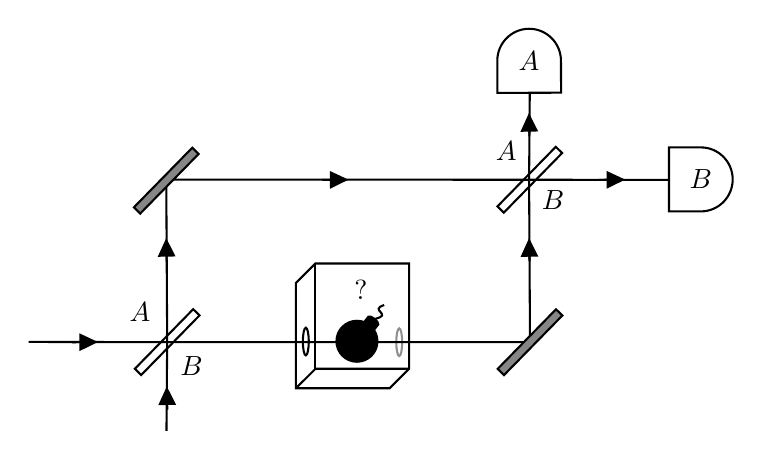
\begin{tikzpicture}[x=0.75pt,y=0.75pt,yscale=-1,xscale=1]
%uncomment if require: \path (0,300); %set diagram left start at 0, and has height of 300

%Shape: Rectangle [id:dp05331443244256162] 
\draw   (232.64,194.14) -- (260.76,165.42) -- (263.8,168.43) -- (235.68,197.15) -- cycle ;
%Straight Lines [id:da6101932312929839] 
\draw    (248.22,181.29) -- (247.88,224) ;


%Straight Lines [id:da37500240484008773] 
\draw    (181.51,181.2) -- (248.22,181.29) ;


%Straight Lines [id:da7395900492947349] 
\draw    (247.78,103.5) -- (248.22,181.29) ;


%Shape: Rectangle [id:dp7145865786703387] 
\draw   (407.34,115.91) -- (435.46,87.19) -- (438.5,90.2) -- (410.38,118.92) -- cycle ;
%Straight Lines [id:da406692659919365] 
\draw    (248.58,181.29) -- (423.03,181.33) ;


%Straight Lines [id:da251128727045983] 
\draw    (248.33,103.01) -- (422.78,103.05) ;


%Straight Lines [id:da6635342486103979] 
\draw    (422.59,103.53) -- (423.03,181.33) ;


%Straight Lines [id:da7433774894582017] 
\draw    (422.92,103.05) -- (489.62,103.14) ;


%Straight Lines [id:da6227633326802493] 
\draw    (422.92,60.82) -- (422.59,103.53) ;


%Shape: Rectangle [id:dp9484177753358207] 
\draw  [color={rgb, 255:red, 0; green, 0; blue, 0 }  ,draw opacity=1 ][fill={rgb, 255:red, 134; green, 134; blue, 134 }  ,fill opacity=1 ] (232.19,116.35) -- (260.32,87.63) -- (263.36,90.64) -- (235.23,119.36) -- cycle ;
%Straight Lines [id:da9162790812582262] 
\draw    (202.27,181.35) -- (212.87,181.26) ;
\draw [shift={(214.87,181.24)}, rotate = 539.49] [fill={rgb, 255:red, 0; green, 0; blue, 0 }  ][line width=0.75]  [draw opacity=0] (8.93,-4.29) -- (0,0) -- (8.93,4.29) -- cycle    ;

%Straight Lines [id:da6345146939842947] 
\draw    (248.27,213.87) -- (248.09,204.64) ;
\draw [shift={(248.05,202.64)}, rotate = 448.87] [fill={rgb, 255:red, 0; green, 0; blue, 0 }  ][line width=0.75]  [draw opacity=0] (8.93,-4.29) -- (0,0) -- (8.93,4.29) -- cycle    ;

%Straight Lines [id:da5741704284114686] 
\draw    (248,142.39) -- (247.82,133.17) ;
\draw [shift={(247.78,131.17)}, rotate = 448.87] [fill={rgb, 255:red, 0; green, 0; blue, 0 }  ][line width=0.75]  [draw opacity=0] (8.93,-4.29) -- (0,0) -- (8.93,4.29) -- cycle    ;

%Straight Lines [id:da9412424001460007] 
\draw    (422.81,142.43) -- (422.63,133.2) ;
\draw [shift={(422.59,131.21)}, rotate = 448.87] [fill={rgb, 255:red, 0; green, 0; blue, 0 }  ][line width=0.75]  [draw opacity=0] (8.93,-4.29) -- (0,0) -- (8.93,4.29) -- cycle    ;

%Straight Lines [id:da16868581259330884] 
\draw    (322.96,103.14) -- (333.56,103.05) ;
\draw [shift={(335.56,103.03)}, rotate = 539.49] [fill={rgb, 255:red, 0; green, 0; blue, 0 }  ][line width=0.75]  [draw opacity=0] (8.93,-4.29) -- (0,0) -- (8.93,4.29) -- cycle    ;

%Straight Lines [id:da32815921714688745] 
\draw    (456.27,103.1) -- (466.87,103) ;
\draw [shift={(468.87,102.99)}, rotate = 539.49] [fill={rgb, 255:red, 0; green, 0; blue, 0 }  ][line width=0.75]  [draw opacity=0] (8.93,-4.29) -- (0,0) -- (8.93,4.29) -- cycle    ;

%Straight Lines [id:da5754252869558345] 
\draw    (422.75,82.18) -- (422.57,72.95) ;
\draw [shift={(422.53,70.95)}, rotate = 448.87] [fill={rgb, 255:red, 0; green, 0; blue, 0 }  ][line width=0.75]  [draw opacity=0] (8.93,-4.29) -- (0,0) -- (8.93,4.29) -- cycle    ;

%Flowchart: Delay [id:dp9432596481685707] 
\draw   (490.01,87.47) -- (505.34,87.47) .. controls (513.81,87.47) and (520.68,94.38) .. (520.68,102.89) .. controls (520.68,111.41) and (513.81,118.31) .. (505.34,118.31) -- (490.01,118.31) -- cycle ;
%Flowchart: Delay [id:dp4563574851197332] 
\draw   (407.32,61.21) -- (407.27,45.79) .. controls (407.24,37.28) and (414.08,30.35) .. (422.55,30.32) .. controls (431.02,30.29) and (437.91,37.17) .. (437.94,45.69) -- (438,61.11) -- cycle ;
%Shape: Rectangle [id:dp6254395580176015] 
\draw  [color={rgb, 255:red, 0; green, 0; blue, 0 }  ,draw opacity=1 ][fill={rgb, 255:red, 134; green, 134; blue, 134 }  ,fill opacity=1 ] (407.45,194.18) -- (435.57,165.46) -- (438.61,168.47) -- (410.49,197.19) -- cycle ;
%Shape: Circle [id:dp013195896602818946] 
\draw  [fill={rgb, 255:red, 0; green, 0; blue, 0 }  ,fill opacity=1 ] (329.77,180.88) .. controls (329.77,175.42) and (334.19,171) .. (339.64,171) .. controls (345.1,171) and (349.52,175.42) .. (349.52,180.88) .. controls (349.52,186.33) and (345.1,190.75) .. (339.64,190.75) .. controls (334.19,190.75) and (329.77,186.33) .. (329.77,180.88) -- cycle ;
%Flowchart: Stored Data [id:dp9468842845409164] 
\draw  [fill={rgb, 255:red, 0; green, 0; blue, 0 }  ,fill opacity=1 ] (349.91,172.79) -- (346.81,176.69) .. controls (347.14,176.28) and (346.34,175.11) .. (345.04,174.07) .. controls (343.74,173.04) and (342.42,172.53) .. (342.09,172.94) -- (345.19,169.04) .. controls (345.51,168.63) and (346.84,169.14) .. (348.14,170.17) .. controls (349.44,171.21) and (350.24,172.38) .. (349.91,172.79) -- cycle ;
%Curve Lines [id:da5409664000175873] 
\draw    (348.14,170.17) .. controls (357.52,167.92) and (345.02,165.92) .. (352.77,163.42) ;


%Shape: Cube [id:dp23004251794331032] 
\draw   (364.78,194.13) -- (355.37,203.53) -- (310.25,203.53) -- (310.25,152.81) -- (319.66,143.4) -- (364.78,143.4) -- cycle ; \draw   (310.25,203.53) -- (319.66,194.13) -- (364.78,194.13) ; \draw   (319.66,194.13) -- (319.66,143.4) ;
%Shape: Ellipse [id:dp3375854777763616] 
\draw   (313.6,181) .. controls (313.6,177.32) and (314.23,174.33) .. (315.02,174.33) .. controls (315.8,174.33) and (316.43,177.32) .. (316.43,181) .. controls (316.43,184.68) and (315.8,187.67) .. (315.02,187.67) .. controls (314.23,187.67) and (313.6,184.68) .. (313.6,181) -- cycle ;
%Shape: Ellipse [id:dp1573514547024959] 
\draw  [color={rgb, 255:red, 0; green, 0; blue, 0 }  ,draw opacity=0.44 ][fill={rgb, 255:red, 0; green, 0; blue, 0 }  ,fill opacity=0 ] (358.6,181.33) .. controls (358.6,177.65) and (359.23,174.67) .. (360.02,174.67) .. controls (360.8,174.67) and (361.43,177.65) .. (361.43,181.33) .. controls (361.43,185.02) and (360.8,188) .. (360.02,188) .. controls (359.23,188) and (358.6,185.02) .. (358.6,181.33) -- cycle ;

% Text Node
\draw (259.93,192.77) node   {$B$};
% Text Node
\draw (235.17,166.66) node   {$A$};
% Text Node
\draw (411.53,89.42) node   {$A$};
% Text Node
\draw (434.19,112.76) node   {$B$};
% Text Node
\draw (505.34,102.89) node   {$B$};
% Text Node
\draw (422.61,45.74) node   {$A$};
% Text Node
\draw (341.6,156) node  [align=left] {?};


\end{tikzpicture}
\end{center}